
\section{Evaluation of register updates}
\label{sec:stt-derivable}
In this section, we deal with the second computation phase in a first-order register transducer, namely evaluating register updates. Together with Proposition~\ref{prop:forat} from the previous section, this completes the proof that all first-order register transducers are derivable. This in turn, together with Theorem~\ref{thm:stt} about expressive completeness of first-order register transducers, completes the proof of our main result. 


When showing derivability of  evaluation for register updates, we  use the language of $\lambda$-calculus.  In Section~\ref{sec:one-register},  we show that evaluation of $\lambda$-terms is derivable, under certain restrictions. This result is then used in Section~\ref{sec:updates-endgame}, where unfolding the matrix power is used to reduce the evaluation of register updates to the evaluation of $\lambda$-terms.  

\section{Evaluation of simply typed linear terms}
\label{sec:one-register}

In this section, we consider an important example of derivable term transformations, namely evaluating (i.e.~computing $\beta$-normal forms of)  simply typed  $\lambda$-terms that are linear in the sense that each bound variable is used exactly once in its scope. Apart from its independent interest, evaluation of $\lambda$-terms will  be used in the proof our main theorem. 



\newcommand{\otype}{o}
We assume that the reader is familiar with the basic notions of the simply typed $\lambda$-calculus; more detailed definitions can be found in~\cite{sorensen_lectures_2006}. Define  \emph{simple types} to be expressions  generated from an atomic type $\otype$ using a binary arrow constructor, as in the following examples:
    \begin{align*}
        \otype \qquad \otype \to \otype \qquad (\otype \to \otype) \to (\otype \to \otype) \qquad \cdots 
    \end{align*}
Let $X$ be a set of variables, each one with an associated simple type.  A $\lambda$-term over these variables can be seen as a tree over the ranked alphabet
\begin{align*}
      \overbrace{\set{x : x \in X}}^{\text{arity 0}} \cup \overbrace{\set{\lambda x : x \in X}}^{\text{arity 1}} \cup  \overbrace{\set @}^{\text{arity 2}}
\end{align*}
where @ is the application symbol that is used to apply one term to another.
We say that a $\lambda$-term is \emph{well-typed} if one can associate  to it  a simple type according to the usual typing rules of simply typed $\lambda$-calculus\footnote{
    Here we assume that the variables are typed, but the types for the remaining $\lambda$-terms need to be inferred. We could adopt a different approach, more thoroughly in the style of Church, where all term constructors (application and $\lambda$-abstraction) come decorated with the type of the resulting term. We do not do this to make  notation lighter, and also because one show -- see the appendix -- that first-order logic is enough to reconstruct the type of a term once the types of the variables are known. 
}, see~\cite[Definition 3.2.1]{sorensen_lectures_2006}. Because the variables are typed, a  $\lambda$-term can have either a unique type, or it is not well-typed.  Here is an example of a well-typed $\lambda$-term: 
\mypic{45}
We use the standard notion of $\beta$-reduction for $\lambda$-terms, see~\cite[Definition 1.2.1]{sorensen_lectures_2006}. 
Because of normalisation and confluence for the simply typed $\lambda$-calculus, every well-typed $\lambda$-term has a unique normal form, i.e~a $\lambda$-term to which it $\beta$-reduces (in zero or more steps), and which cannot be further $\beta$-reduced.


\begin{example}\label{ex:exponential}
    Because of iterated duplication, the normal form of a $\lambda$-term can be exponential. Assume that we have two variables $\typevar x  \otype$ and $\typevar y {\otype \to \otype \to \otype}$ and consider the $\lambda$-terms defined by:
    \begin{align*}
        M_0 \eqdef \typevar x \otype \qquad M_{n+1} = (\lambda \typevar x  \otype . \typevar y {\otype \to \otype \to \otype}  \typevar x  \otype \typevar x  \otype)M_n.
    \end{align*}
    The $\lambda$-term $M_n$ is well-typed and of type $\otype$. It has size linear in $n$, but its normal form has size exponential in $n$. 
    % as shown in the following picture, which uses variables $x : \otype$ and  $z : \otype \to \otype \to \otype$.
    % \mypic{44}
\end{example}
As witnessed by the above example, normal forms can be exponential size (or worse, see~\cite[Section 3.6]{sorensen_lectures_2006}), and therefore they cannot be computed  using derivable functions or first-order transductions, because the latter have linear size outputs. To avoid this problem, we  limit attention to linear $\lambda$-terms: a $\lambda$-term is called \emph{linear} if every bound variable is used exactly once in its scope. Here is an example: 
\mypic{43}
For linear $\lambda$-terms, each step of $\beta$-reduction reduces the number of nodes by exactly 3, and therefore the normal form is linear in the size of (in fact, smaller or equal to) the original term. 

Linearity alone is not enough to normalise terms with first-order transductions. Another obstacle is terms that use types of unbounded complexity, as illustrated in the following example. 

\begin{example}
Consider the following $\lambda$-terms, which have types of unbounded size:     \begin{align*}
        M_0 \eqdef \typevar u {\otype \to \otype}  \qquad M_{n+1} \eqdef \overbrace{\lambda \typevar x {\otype}. \lambda \typevar y {\otype}.   M_n (\typevar z {\otype \to \otype \to \otype}  \typevar x {\otype} \typevar y {\otype}).}^{\text{type} \overbrace{\otype \to \otype \to \cdots \to \otype}^{\text{$n+1$ arrows}}}
    \end{align*}
    Apart from having large types (although still of rank 1, as described in~\cite[Exercise 3.6.7]{sorensen_lectures_2006}), these  $\lambda$-terms are simple: they use four variables (although the bound variables are reused), and are linear, because each bound variable is used exactly once in its scope. 
    To $M_n$, apply  $m$ arguments of type $\otype$:
    \begin{align}\label{eq:complicated-term}
    M_n \overbrace{\typevar v \otype \ \typevar v {\otype} \cdots \typevar v{\otype} }^{\text{$m$ times}}.
    \end{align}
    We claim that the above $\lambda$-term cannot be normalised using a first-order transduction, or even a monadic second-order transduction. In order to normalise, a transduction would need to be able to compare the numbers $n$ and $m$ as follows:  if $m < n$  the normal form contains $\lambda$, if $m=n$  the normal form does not contain $\lambda$, and if $m > n$ then the normal form is undefined because the $\lambda$-term is not well-typed.  Whether or not a $\lambda$-term (seen as a tree over a finite alphabet) contains $\lambda$ is a first-order definable property, and first-order definable properties are preserved under inverse images of first-order transductions. Therefore, if normalisation would be a first-order transduction,
then there would be a first-order formula which would be true for terms of the form~\eqref{eq:complicated-term} with $m>n$ and which would be false for terms of the form~\eqref{eq:complicated-term} with $m=n$. Such a formula cannot exist (even if we allow monadic second-order logic), which can be shown using a pumping argument or Ehrenfeucht-Fra\"iss\'e games. 
\end{example}

The above example explains why we need to bound the size of types that occur in subterms, motivating the following definition:  we say that a $\lambda$-term uses only types from a finite set of simple types $\typeset$ if all  subterms have types in $\typeset$.  Once we assume that $\lambda$-terms are linear, use a fixed finite set of bound variables, and use only types from a fixed finite set of simple types, then normalisation can be done by a derivable function, and therefore also by a first-order tree-to-tree transduction: 

\begin{theorem}\label{thm:normalise} Let $X$ be a finite set of simply typed variables, and let $\typeset$ be a finite set of simple types.
    The following tree-to-tree function is derivable (i.e.~it is the tree restriction of a derivable function on terms):
    \begin{align*}
        M \in \text{$\lambda$-terms over variables $X$} \qquad \mapsto \qquad \begin{cases}
            \text{normal form of $M$} & \text{if $M$ is linear, well-typed,}\\
            & \text{and uses only types from $\typeset$;}\\
            M & \text{otherwise}.
        \end{cases}
    \end{align*}
\end{theorem}

% Actually, we prove a stronger result, namely that the above function is derivable. In the end, of course, we will prove that all first-order tree-to-tree transductions are derivable, but our proof of this fact will use the derivability of normalisation as stated in Theorem~\ref{thm:normalise}.



% Recall that elements of $\tmonad \rSigma$ are defined to be trees over $\rSigma + \varnames$, where 
% \begin{align*}
%     \varnames = \set{x_1,x_2,\ldots}
% \end{align*}
% is a fixed set of  variable names that are used for ports. In this section, we view $\varnames$ as a simply typed set, where all variables $x_1,x_2,\ldots$ have the same simple type $\otype$.  Under this convention, we can view
% \begin{align*}
%     \tmonad (\overbrace{\set{x : x \in X}}^{\text{arity 0}} \cup \overbrace{\set{\lambda x : x \in X}}^{\text{arity 1}} \cup  \overbrace{\set @}^{\text{arity 2}})
% \end{align*}
% as a set of $\lambda$-terms. This is exactly the set of those $\lambda$-terms over variables $X + \varnames$ where: (a) variables from $\varnames$ are never bound; and (b) there is some $n$ such that each of the variables $x_1,\ldots,x_n \in \varnames$  appears as a free variable exactly once  and the remaining variables in $\varnames$ do not appear at all. If $S$ is a finite set of simple types, then define  $\linterm S X$ to be those terms in .. which are linear and $S$-typed. 

% Computing the normal form is beyond the scope of first-order transductions, the principal reason being that first-order transductions have linear size outputs, while normalisation can incur a blowup that is exponential or larger,
%  In Section~\ref{sec:lambda}, we will show that normalisation can be computed by a first-order transduction, assuming that: (a) the input terms are linear, which means that each bound variable is used exactly once in its scope; (b) we place an upper bound on the complexity of types used in subterms. 

% as discussed in Example~\ref{ex:labmda-terms}.  We show that the tree-to-tree function which inputs a  term and outputs its normal form can be derived, assuming that bound variables are used exactly one and there is a bound on the number of distinct terms types that can appear in the term. 

% Let $X$ be a typed set, i.e.~a set of variables with associated simple types. As in  Example~\ref{ex:labmda-terms},  we view $\lambda$-terms with variables of $X$ as trees over an ranked alphabet $\lamrank X$. 

% \begin{lemma}
%     For every typed set $X$ and every finite set $S$ of simple types, the tree language 
%     \begin{align*}
%         \set{ M \in \trees \lamrank X : \text{$M$ is well-typed and all subterms have type in $S$}}
%     \end{align*}
%     is first-order definable 
% \end{lemma}



% We say that a function $\ranked f : \linterm S X \rto \linterm S Y$ is \emph{derivable} if it can be extended to a derivable function $\ranked g : \tmonad \lamrank X \rto \tmonad \lamrank X$. The main result of this section is that normalisation is derivable, for every fixed finite $X$ and $S$. 
% \begin{proposition}\label{prop:one-register} 
%     For every typed set $X$ and every finite set $S$ of simple types, the function 
%     \begin{align*}
%         M \in  \linterm S X \qquad \mapsto \qquad \text{normal form of $M$} \in  \linterm S X
%     \end{align*}
%     is derivable.
% \end{proposition}
%
Generalize to non pure lambda terms.

\subsection{Evaluation of register updates}
\label{sec:updates-endgame}
In this section, we complete the proof of derivability for the evaluation of register updates. The rough idea is to reduce it to the evaluation of $\lambda$-terms as in Theorem~\ref{thm:normalise}. %This reduction will involve the matrix power. 

Fix a first-order register transducer, with registers names $\regnames$ and output alphabet $\rGamma$. We suppose that it has $k$ registers and the set of names $\regnames$ is $[1,k]$. In this case, register valuations and register updates can be though of as lists of terms. 
From now on, when speaking about register updates or register valuations, we assume these register names and this alphabet. Our goal is to prove the following lemma. 
\begin{lemma}\label{lem:derive-register-updates}
    The  following tree-to-tree function  is derivable:
    \begin{eqnarray*}
    \trees{\ranked{\text{(register updates)}}} &\to & \trees \rGamma \\
    t & \mapsto & \text{contents of the output register}\\
    && \text{after evaluating $t$}
    \end{eqnarray*}    
\end{lemma}

As discussed at the beginning of  Section~\ref{sec:stt}, the lemma completes the proof  our main result, Theorem~\ref{thm:main}.  




The main ingredient to prove the lemma consists in defining an arity preserving function, called \emph{$\lambda\text{-representation}$}, which encodes register updates as a matrix power of $\lambda$-terms. 

\paragraph*{$\lambda$-representations of register updates.} If $m$ is the maximal arity of the registers $\regnames$, let $X=\set{x_1\dots,x_m}$ be a set of variables of type $\otype$.  We set $\ranked{\Gamma_\lambda}$ to be the type $\ranked{\Gamma+X^\lambda}$. The     $\lambda$-representation of register updates is an  arity preserving function, of type
\begin{align}\label{eq:lambda-representation-regup}
\ranked{
    \xymatrix@C=2cm{
 \text{register updates}    \ar[r]^-{\text{$\lambda$-representation}} &
 \mati k {(\tmonad\Gamma_\lambda)}
}
}.
\end{align}
To define it, we use the auxiliary function $\lambda$ of type
\begin{align*}
\lambda: \ranked{\tmonad(\Sigma+n R)} \to \ranked{\tmonad \Gamma_\lambda} 
\end{align*}
defined as follows. If  $t$ be a term of $\ranked{\tmonad(\Sigma+n R)}$ of arity $l$, then $\lambda(t)$ is obtained by:
\begin{enumerate}
\item[(a)] Replacing the  $i$-th port  of $t$ with the variable $x_i$.
\item[(b)] Binding all the  variables $x_1,\ldots,x_l$  at the beginning of the term, in this order.
\item[(c)] Applying the following rewriting rule, where $r_i \in \ranked{nR}$
\begin{align*}
r_i(t_1,\dots,t_p) \mapsto @(@(\dots @(\portletter, t_1)\dots,t_{p-1}),t_p)
\end{align*}
which replaces every $p$-ary letter $r_i$ by a spine of $@$ of lenght $p$.
This rewriting rules creates, for every name $r_i$, a new port. We call it the \emph{port of $r_i$}.
\end{enumerate}
This construction is is illustrated by the following picture.
\begin{center}
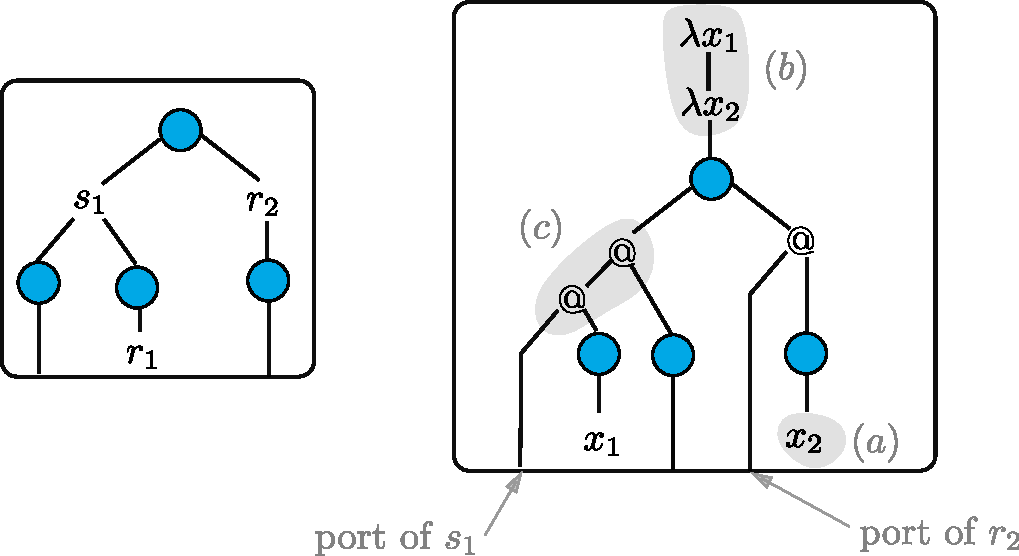
\includegraphics[scale=.33]{pictures/lambda}
\end{center}
Note that the function $\lambda$ is not arity preserving. Now, the $\lambda$-representation function is defined by
\begin{align*}
u \mapsto \lambda(u)/f 
\end{align*}
 $f$ being the function
 \begin{align*}
 \text{port of $r_i$ } \mapsto (r,i).
 \end{align*}


The following example illustrates $\lambda$-representations in the case where we have two registers. To avoid the ambiguities, registers $1$ and $2$ are named $r$ and $s$ respectively in the figure.
\begin{center}
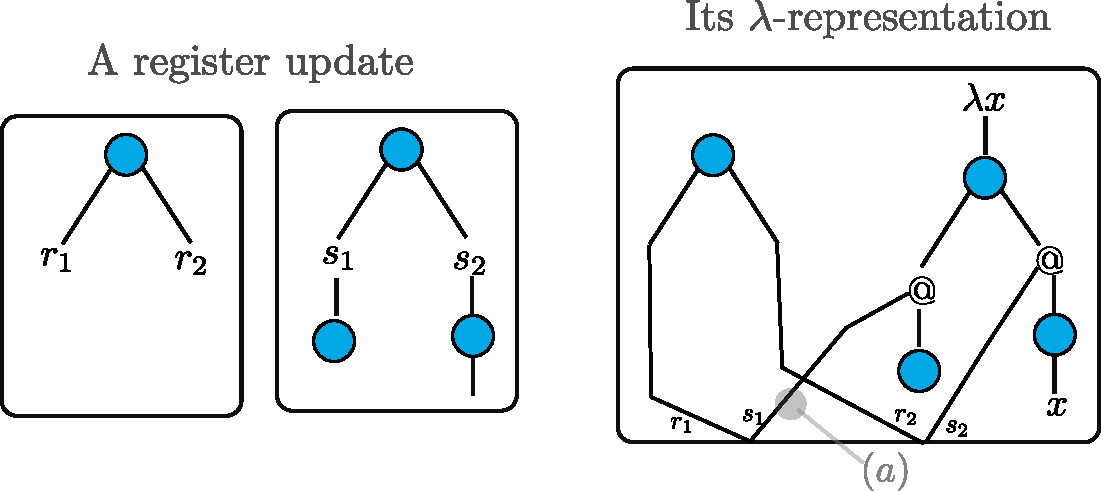
\includegraphics[scale=.33]{pictures/lambda-rep}

\noindent {\small (a): port of $s_1$ contributes to the second position of the first port in the matrix power.}
\end{center}
Before showing how $\lambda$-representation will be used to evaluate register updates,  let us notice that it has 3 main properties.
\begin{itemize}
\item It is an arity preserving function. Since its domain is finite, it is a prime function.
\item A register update is monotone (in the sense Definition~\ref{def:stt}) if and only if its $\lambda$-representation is monotone (in the sense of matrix power as defined in  Section~\ref{sec:unfolding}). It follows that the $\lambda$-representation produces only monotone elements of the matrix power, if it is applied to register updates that come from a first-order register transducer. 
This will ensure that we can use the monotone unfolding operation. 
\item $\lambda$-representation outputs (matrix powers of) $\lambda$-terms which are  linear and can be typed using a bounded set of types, namely $\otype$ and $\otype\to \otype$. It falls therefore under the scope of Theorem~\ref{thm:normalise}.
\end{itemize}

 
%To get the feeling of this function, we will first present it in the case where the automaton has only one unary regiTheorem~\ref{thm:normalise}.ster. The general case will be presented  in a second step.
%
%\paragraph*{The case of one register (k=1).} There is mismatch between the arity of register updates and the arity of the terms they contain (which is always 1). This is illustrated by the left figure below: the register update is of arity 2, but its content is of arity 1. A consequence of this mismatch is that a term of register updates cannot be seen as a term of terms, and the prime function of flattening and block etc cannot be applied; in other words, the inner structure of register updates is not accessible.
%Let us fix a variable $x$ of type $o$. The $\lambda$-representation, described in the figure below, is intended to bridge this gap, while preserving the behavior of register updates. 
%\begin{center}
%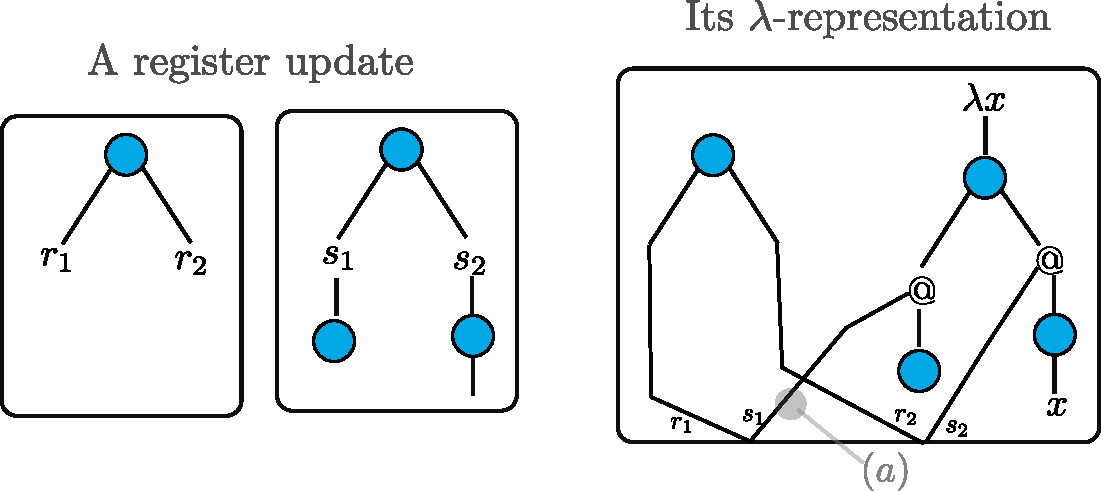
\includegraphics[scale=.36]{pictures/lambda-rep}
%\end{center}
%In words, the $\lambda$-representation transforms the (unique) port of the inner term into $x$ and replaces every letter $r_i$ is by a redex, the pending port of this redex becomes \begin{figure}[]
    
%
%The $\lambda$-representation does not only match the arities between the register update and their content, it also  respects their behavior, as illustrated by the following diagram.
%\begin{center}
%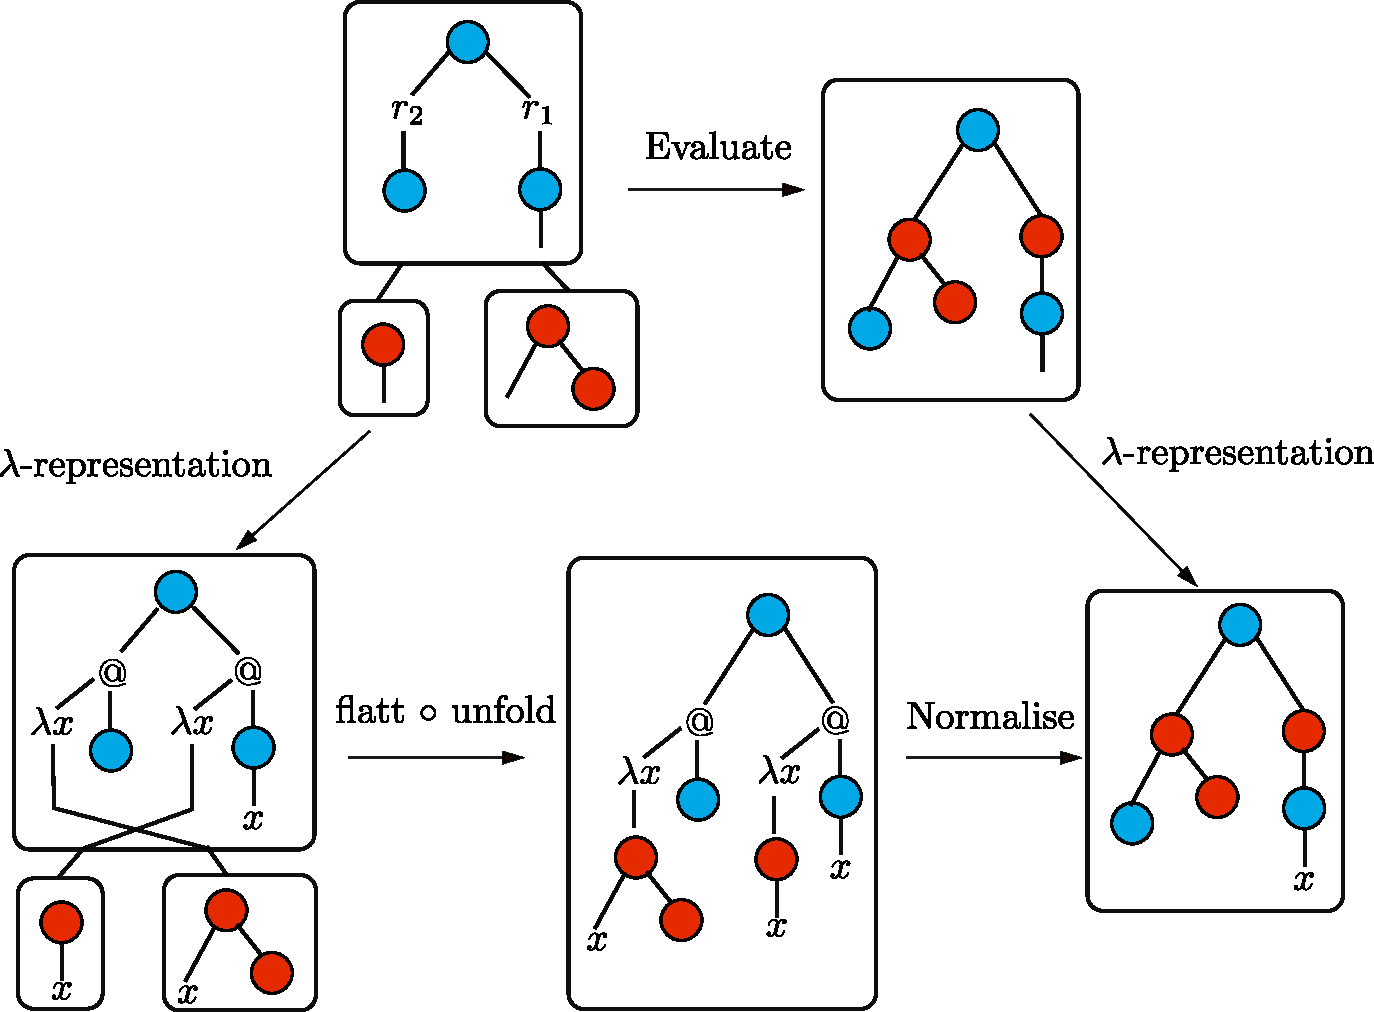
\includegraphics[scale=.36]{pictures/lambda-rep-diagram}
%\end{center}
%In words, the evaluation of a term of register updates can be simulated, through  $\lambda$-representation, by unfolding and normalization functions, which are derivable. 
%
%\paragraph*{The general case.} Let us describe the $\lambda$-representation in the general case. As in the case $k=1$, the inner portes become the variable $x$, every register name becomes a redex. The issue here is how to combine the ports.
%
%\begin{center}
%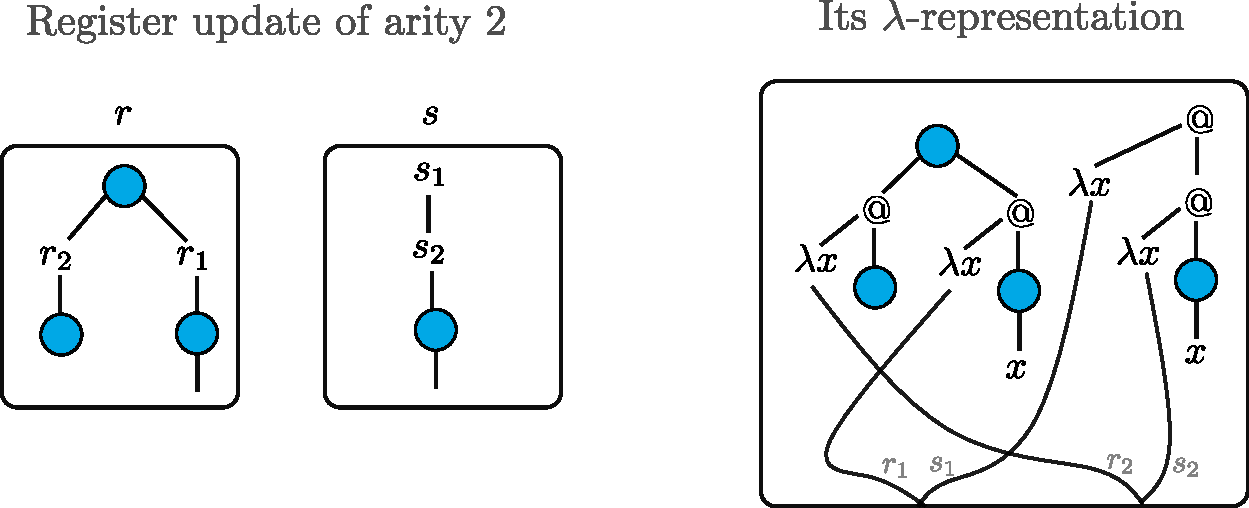
\includegraphics[scale=.36]{pictures/lambda-rep-general}
%\end{center}
% To describe the register updates in a transducer, we will use notions from $\lambda$-calculus.  
% We will also give more precise description of the $\lambda$-calculus in Section~\ref{sec:one-register}; for the moment it is enough to assume that $\lambda$-terms are like trees, except that they allow variables $x,y,z,\ldots$; binding the variables using $\lambda x, \lambda y, \lambda z, \ldots$ and applying one term to another. The evaluation of $\lambda$-terms is performed by $\beta$-reduction
% \begin{align*}
% (\lambda x. M) N \qquad \to_\beta \qquad M[x:=N],
% \end{align*}
% which substitutes a variable by an argument. The $\lambda$-terms that we use are going to be simply typed, which will imply that $\beta$-reduction eventually terminates, arriving at a normal form (called the value of the $\lambda$-term), and this normal form will not depend on the order in which $\beta$-reduction was performed. 
% Define a \emph{$\lambda$-term} to be an expression built using the following grammar
% \begin{align*}
%  \underbrace{x,y,z,\ldots}_{\text{variables}} \quad \underbrace{MN}_{\text{application}} \quad \underbrace{\lambda x.M}_{\text{$\lambda$-abstraction}}.
% \end{align*}
% We use simply typed $\lambda$-calculus. This means that every variable is associated to a type, and we only consider terms which are well-typed. The types that we use are simple types: these 
% Sometimes, we extend the syntax, by allowing a symbols from the output alphabet  $\rGamma$:  terms of the form $a(M_1,\ldots,M_n)$, where $a \in \rGamma$ is a symbol of arity $n$. 

%The red circles in the above picture, which represent nodes of the input term, can be seen  as syntactic sugar: a node with a label  $a \in \rGamma$ of arity $n$ is represented  as a variable of type 
%\begin{align}\label{eq:low-order-type}
%\overbrace{\otype \to \otype \to \cdots \to \otype}^{\text{$n$ times}} \to \otype
%\end{align}
%applied to $n$ arguments. The variables corresponding to $\rGamma$  -- which are not bound -- are the only ones used multiple times; every other variable is used at most once in its scope.   Furthermore, all sub-terms in the $\lambda$-representation have type of the form~\eqref{eq:low-order-type}, with $n$ being at most the maximal arity of letters in $\rGamma$. Summing up, the $\lambda$-representation is affine and can be typed using a bounded set of types, and therefore it falls under the scope of Theorem~\ref{thm:normalise}.

%As discussed in Section~\ref{sec:one-register}, the $\lambda$-representation of a term in $\rGamma$ can be seen as a tree over a finite ranked alphabet; call this ranked alphabet $\ranked{\Gamma_\lambda}$. When the outputs are viewed as trees, the function
%\begin{align}\label{eq:lambda-representation-term}
%\xymatrix@C=2cm{
%    \tmonad \rSigma 
%    \ar[r]^{\text{$\lambda$-representation}} &
%    \trees {\ranked{\Gamma_\lambda}}
%}
%\end{align}
%is not arity-preserving, since all outputs have arity zero. For tree inputs, $\lambda$-representation is the identity function. 

%\paragraph*{The $\lambda$-representation of register updates.} To represent register updates using $\lambda$-terms, we use  the $k$-th matrix power, where  $k$ is the number of registers. The     $\lambda$-representation of register updates is an  arity preserving function, of type
%\begin{align}\label{eq:lambda-representation-regup}
%\ranked{
%    \xymatrix@C=2cm{
% \text{register updates}    \ar[r]^-{\text{$\lambda$-representation}} &
% \mati k {(\tmonad\Gamma_\lambda)}
%}
%}.
%\end{align}
%This function is illustrated in Figure~\ref{fig:labmda-representation-for-register-updates}. 
% \miktodo{Give a definition, maybe?}
%Although most likely this  function is not derivable in general;  it does become derivable if we restrict the domain to a finite set of register updates, by virtue of having a finite domain.





\label{page:monotone-discussed}


\paragraph*{Putting it all together.}
Having defined the $\lambda$-representation for terms and register updates, we now observe  that the semantics of a register automaton are translated -- under $\lambda$-representation -- to unfolding the matrix power and evaluating a $\lambda$-term.  This observation is illustrated in Figure~\ref{fig:register-lambda} and stated in the following lemma.
\begin{figure}[]
    \centering
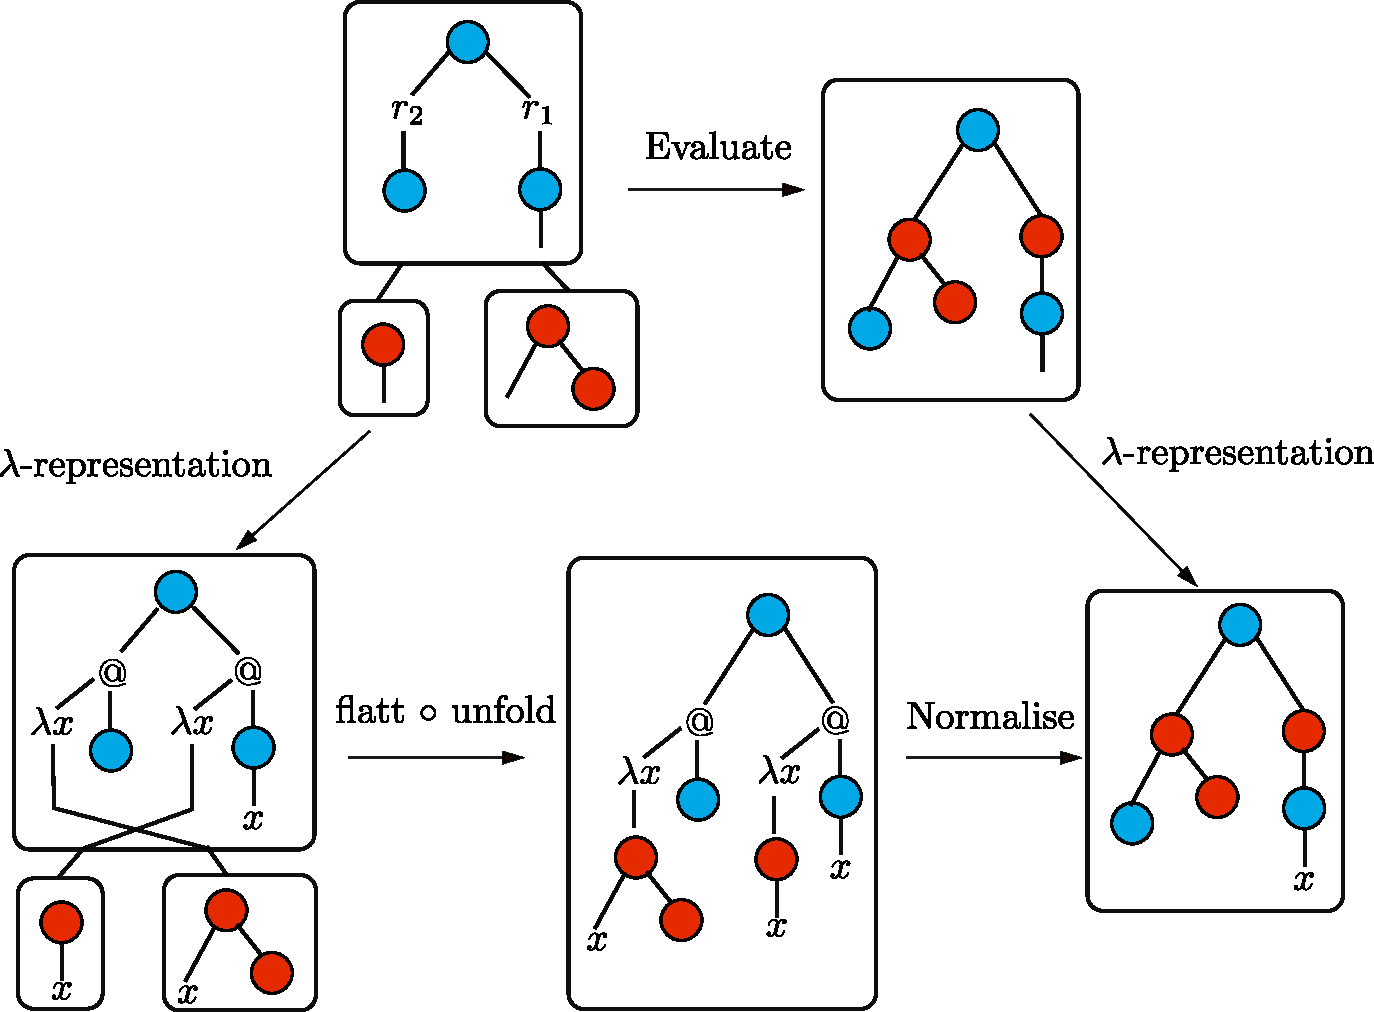
\includegraphics[scale=.3]{pictures/lambda-rep-diagram}   
    \caption{Evaluation of register updates can be simulated, through $\lambda$-representation, by unfolding of matrix power folloed by normalisation of $\lambda$-terms.}
    \label{fig:register-lambda}
\end{figure}


\begin{lemma}
    The following diagram commutes 
        \captionsetup{singlelinecheck=false}
    \centering
    \xymatrix@C=3cm{
        \trees \ranked{\text{(register updates)}} 
        \ar[dd]_{\substack{\text{evaluate}\\\text{register}\\\text{updates}}}^{\text{(a)}}
        \ar[r]^-{\trees(\text{\ranked{$\lambda$-representation}})}_{\text{(c)}}
        &
        \trees \ranked{(\mati k{(\tmonad \Gamma_\lambda)})}
        \ar[d]^{\substack{\text{unfold}\\\text{matrix}\\\text{power}}}_{\text{(d)}} \\
        & 
        (\trees \ranked{\Gamma_\lambda})^k 
        \ar[d]^{\substack{\text{evaluate}\\\text{$\lambda$-terms}}}_{\text{(e)}}\\
         \text{register valuations}
        \ar[r]_-{\text{$\lambda$-representation}}^{\text{(b)}}
        &
        (\trees \ranked{\Gamma_\lambda})^k
    }    
%    \caption[foo bar]{In the diagram, the arrows describe the following operations:
%    \begin{enumerate}
%        \item[(a)] is as defined in the semantics of register transducers; 
%        \item[(b),(c)]   is $\lambda$-representation of register updates as defined in~\eqref{eq:lambda-representation-regup};
%        \item[(d)] is the unfolding as described in Section~\ref{sec:prime-and-combinators}; 
%        \item[(e)] is computing the $\beta$-normal form for each $\lambda$-term.
%    \end{enumerate}
%       }
\end{lemma}

The lemma follows  directly from the definitions, and is given without proof.  
We claim that all of the arrows (c), (d) and (e) on the  right-down path  in the diagram from Lemma~\ref{}  are derivable:
\begin{itemize}
    \item[(c)] Since we are working with a fixed register transducer, there is a finite set of register updates that it uses, and we only need to compute the $\lambda$-representation for those updates. It follows that operation (a) in the figure, when restricted to the finite set of register updates used by the transducer, is derivable.
    \item[(d)] Arrow (d) represents the unfolding of the matrix power. As we have argued before, the outputs of arrow (c) are monotone, and therefore we can use the monotone unfolding operation, which is a  prime function and therefore derivable. There is one technicality that needs to be explained about arrow (d). After applying (monotone) unfolding to the output of arrow (c), we get an  arity zero element of 
    \begin{align*}
        \ranked{
            \mati k {(\tmonad \rGamma_\lambda)}} = \reduce  k {\powersmall{(\tmonad \rGamma_\lambda)}{k}}.
    \end{align*}
    To convert this output into a tuple of trees, we use the last prime function in Figure~\ref{fig:monad} to remove the fold $\reduce k$.
    \item[(e)] Finally, arrow (e) represents the evaluation of $\lambda$-terms. This arrow is derivable thanks to Theorem~\ref{thm:normalise}. The assumptions of this theorem are met, as discussed when describing the $\lambda$-representation.
\end{itemize}
Since arrows (c), (d), (e) are derivable, and the diagram commutes, it follows that  the composition of the arrows (a) and (b) is derivable. In other words, there is a derivable function which maps a tree of register updates to the $\lambda$-representation of the resulting register valuation. If we project the register valuation to the coordinate of the output register, we get the $\lambda$-representation of the output tree, which is the same thing as the output tree, since $\lambda$-representation does nothing for terms of arity zero. 

This completes the proof of Lemma~\ref{lem:derive-register-updates}, and therefore also of the main theorem. 




